\documentclass[12pt,a4paper]{article}

\usepackage[margin=2.2cm]{geometry}
\usepackage{fontspec}
\usepackage{xeCJK}
\setmainfont{Times New Roman}
% 標楷體（Windows 字型名為 DFKai-SB）
\setCJKmainfont{DFKai-SB}[AutoFakeBold,AutoFakeSlant]
\usepackage{amsmath,amssymb,bm}
\usepackage{graphicx}
\usepackage{wrapfig}
\usepackage{setspace}
\usepackage{hyperref}
\usepackage{caption}
\setstretch{1.08}
\raggedbottom
\setlength{\intextsep}{8pt plus 2pt minus 2pt}
\setlength{\textfloatsep}{10pt plus 2pt minus 2pt}

\hypersetup{colorlinks=true,linkcolor=black,urlcolor=blue}
\captionsetup{font=small,labelfont=bf,skip=4pt}
\graphicspath{{figures/}}

\title{\textbf{Control System Homework 01}\\[0.35em]
\large Unit 2: Dynamic Models\\[0.5em]
Problem~3（2.19）電容式麥克風建模}
\author{許楷翊 \quad B13901040}
\date{2026 年 9 月}

\begin{document}
\maketitle

這題是電容麥克風（圖~\ref{fig:schematic}）。下面依 (a)(b)(c) 建模，
並說明作業把靜電力写成 \(f_e\operatorname{sgn}(\dot{x})\) 為什麼不合理。

%==============================================================================
\section{系統在做什麼}

極板 \(a\) 固定，極板 \(b\)（質量 \(M\)）用彈簧 \(K\)、阻尼 \(B\) 接在牆上。
聲音的力 \(f_s(t)\) 推 \(b\)。兩板是電容器，間距 \(x\)，再串 \(L\)、\(R\) 和電壓源 \(v\)。

\begin{wrapfigure}{r}{0.46\textwidth}
  \centering
  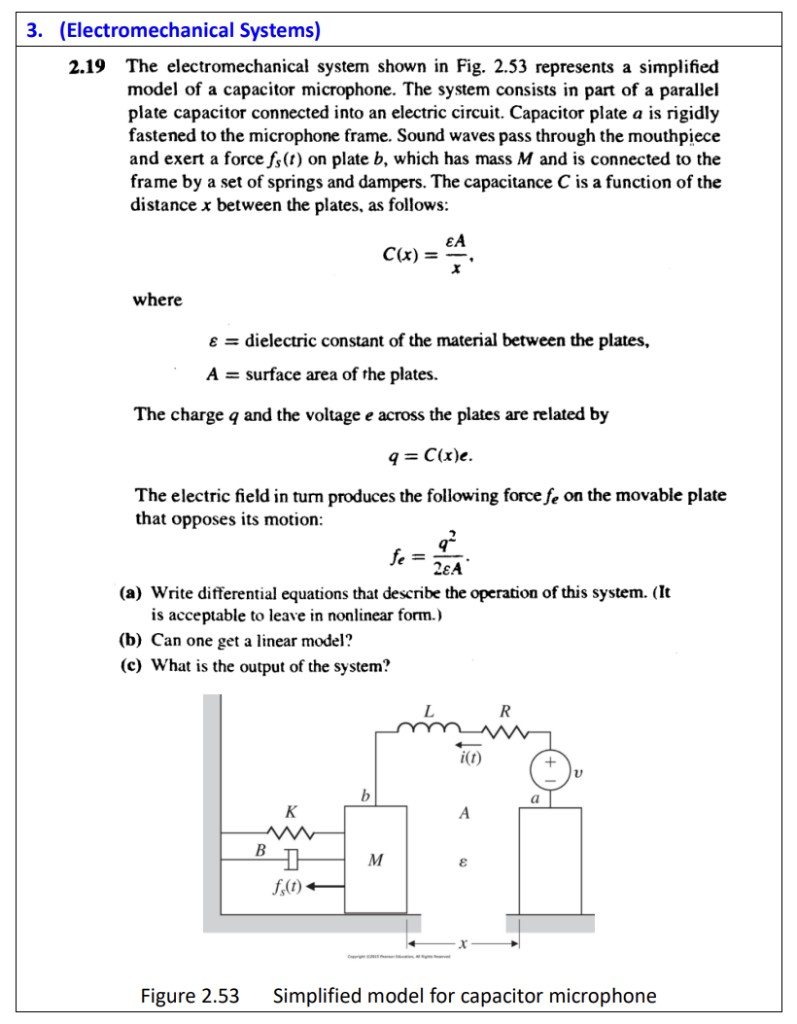
\includegraphics[width=0.44\textwidth]{fig_schematic.png}
  \caption{Fig.~2.53　電容麥克風簡圖。}
  \label{fig:schematic}
\end{wrapfigure}

題目給
\begin{equation}
  C(x)=\frac{\varepsilon A}{x},\qquad
  q=C(x)\,e,\qquad
  f_e=\frac{q^2}{2\varepsilon A}.
\label{eq:given}
\end{equation}
\(x\) 愈小，電容愈大。\(f_e\) 是兩板之間的電力。
題目說它 “opposes its motion”。

座標：\(x\) 是兩板距離，變大代表 \(b\) 往左、兩板分開。
\(f_s>0\) 讓 \(x\) 變大。電源用直流偏壓 \(V_0\)（真的麥克風也要偏壓才有電訊號）。

%==============================================================================
\section{\(f_e\) 該往哪推？}
\label{sec:fe}

這就是一顆電容器：\(b\) 帶 \(+q\)，\(a\) 帶 \(-q\)，極性永遠相反。
力裡有 \(q^2\)，所以
\[
f_e=\frac{q^2}{2\varepsilon A}\ge 0.
\]
異號相吸：電力永遠把 \(b\) 拉向 \(a\)，也就是永遠讓 \(x\) \textbf{變小}，
和速度 \(\dot{x}\) 無關。\(q=0\) 時力是 0，但不會相斥。

作業解答（圖~\ref{fig:fbd}）却写成
\begin{equation}
  M\ddot{x}+B\dot{x}+Kx+f_e\operatorname{sgn}(\dot{x})=f_s(t),
\label{eq:sgn}
\end{equation}
等於把 “opposes its motion” 當成「力和速度永遠反向」，變成摩擦，不是吸引力。

\begin{figure}[ht]
  \centering
  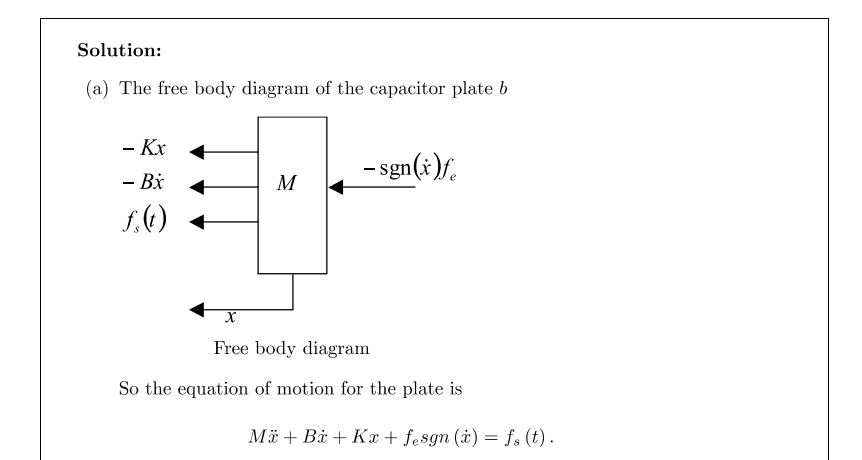
\includegraphics[width=0.42\textwidth]{fig_fbd_sol.png}
  \caption{作業解答的受力圖：\(f_e\) 乘了 \(\operatorname{sgn}(\dot{x})\)。}
  \label{fig:fbd}
\end{figure}

這樣有三個問題：
\begin{enumerate}
  \item \textbf{停著也該有力。}
        \(\operatorname{sgn}(0)=0\)，一靜止電力就消失。充電的兩板停著仍該互吸。
  \item \textbf{靠近時該吸，不該推。}
        \(\dot{x}<0\)（兩板靠近）時，\eqref{eq:sgn} 變成相斥。異號電荷靠近應更吸。
  \item \textbf{這是守恆力，不是阻尼。}
        拉開極板要做功；靠近時電場會幫忙。功率可正可負。
        \(\operatorname{sgn}\) 讓功率永遠 \(\le 0\)，把電力當成摩擦。
\end{enumerate}

“opposes its motion” 比較合理的意思是：\textbf{要把兩板拉開，得先勝過吸引力}，
不是力和 \(\dot{x}\) 永遠反向。

所以正確的力學式是
\begin{equation}
  M\ddot{x}+B\dot{x}+K\bigl(x-x_{\mathrm{rest}}\bigr)+f_e=f_s(t),
\label{eq:mech}
\end{equation}
\(f_e\) 永遠讓 \(x\) 變小。\(x_{\mathrm{rest}}\) 是彈簧沒受力時的間距。

%==============================================================================
\section{電路}

繞一圈：電壓源、電阻、電感、再回到電容，
\begin{equation}
  L\dot{i}+Ri+e=V_0,\qquad
  e=\frac{qx}{\varepsilon A},\qquad
  i=\dot{q}.
\label{eq:kvl}
\end{equation}

%==============================================================================
\section{(a) 非線性方程組}

未知數用 \(x,\dot{x},q,i\)：
\begin{equation}
\begin{aligned}
  \ddot{x}&=\frac{1}{M}\Bigl[f_s(t)-\frac{q^2}{2\varepsilon A}
           -K\bigl(x-x_{\mathrm{rest}}\bigr)-B\dot{x}\Bigr],\\
  \dot{q}&=i,\\
  \dot{i}&=\frac{1}{L}\Bigl(V_0-Ri-\frac{qx}{\varepsilon A}\Bigr).
\end{aligned}
\label{eq:nlin}
\end{equation}
後面模擬就是直接數值積分這組式子，沒有先線性化。

%==============================================================================
\section{(b) 可不可以線性化？}

可以，但要在\textbf{有偏壓的平衡點}附近，對小的聲音線性化。

\(f_s=0\)、速度和電流都是 0 時，平衡 \((x_0,q_0)\) 滿足
\begin{equation}
  q_0=\frac{\varepsilon A V_0}{x_0},\qquad
  K(x_0-x_{\mathrm{rest}})+\frac{q_0^2}{2\varepsilon A}=0.
\label{eq:eqpt}
\end{equation}
彈簧要拉住一直存在的吸引力，所以 \(x_0<x_{\mathrm{rest}}\)（兩板比沒加電時更近）。
若用 \(\operatorname{sgn}\)，靜止時 \(f_e=0\)，平衡會被錯放在 \(x_{\mathrm{rest}}\)。

令 \(x=x_0+\delta x\)，\(q=q_0+\delta q\)，略去二次項：
\begin{equation}
\begin{aligned}
  M\delta\ddot{x}+B\delta\dot{x}
  +\Bigl(K-\frac{q_0^2}{\varepsilon A x_0^2}\Bigr)\delta x
  +\frac{q_0}{\varepsilon A}\,\delta q
  &=\delta f_s,\\
  L\delta\ddot{q}+R\delta\dot{q}
  +\frac{x_0}{\varepsilon A}\,\delta q
  +\frac{q_0}{\varepsilon A}\,\delta x
  &=0.
\end{aligned}
\label{eq:lin}
\end{equation}
靜電會讓等效彈簧變軟。聲音很小，\eqref{eq:nlin} 會接近 \eqref{eq:lin}；
聲音太大就不是線性，甚至可能被吸死（pull-in）。

作業解答寫：\(\operatorname{sgn}\)、\(q^2\) 和 \(qx\) 讓人無法得到有用的線性模型。
這三項不該捆在一起。\(\operatorname{sgn}(\dot{x})\) 在 \(\dot{x}=0\) 不可微，的確不適合一般線性化。
但 \(q^2\) 和 \(qx\) 處處可微：在 \(q_0\neq 0\) 的偏壓點，
\[
\delta(q^2)=2q_0\delta q,\qquad
\delta(qx)=q_0\delta x+x_0\delta q,
\]
就是 \eqref{eq:lin}。若硬繞 \(q=0\) 線性化，這兩項的一階機電耦合都是 0，偏壓麥克風也會沒輸出。
所以：拿掉 \(\operatorname{sgn}\) 是必要的，還要在 \((x_0,q_0)\) 上線性化，才有 useful 的線性模型。

%==============================================================================
\section{(c) 輸出是什麼？}

輸出是電流 \(i(t)\)（或電阻電壓 \(Ri\)），不是間距 \(x\)。
偏壓下 \(q\approx C(x)V_0\)，所以
\begin{equation}
  i=\dot{q}\approx -\frac{\varepsilon A V_0}{x^2}\,\dot{x}.
\label{eq:i}
\end{equation}
\(i\) 跟\textbf{速度}有關。因此：
\begin{itemize}
  \item 階躍：\(x\) 停在新位置後，\(i\to 0\)（沒有直流輸出）；
  \item 脈衝：\(x\) 晃完回到原位，\(i\) 只在晃的時候有值；
  \item 正弦：\(x\) 和 \(i\) 都持續振盪。
\end{itemize}
電容麥克風本來就只對「有在變的聲音」有輸出。

%==============================================================================
\section{模擬結果}

用歐拉法積分 \eqref{eq:nlin}。參數有放大，方便畫面上看得出來，方程式和題目一樣。
輸入可選 step、impulse（短脈衝代替 \(\delta(t)\)）或正弦。

\subsection{脈衝}

圖~\ref{fig:impulse}：\(t=1\,\mathrm{s}\) 敲一下。\(x\) 離開平衡再回來；
\(i\) 出現一個脈衝後變 0，形狀跟 \(\dot{x}\) 一樣。青色 \(f_e\) 幾乎不變，一直是吸引力。

\begin{figure}[ht]
  \centering
  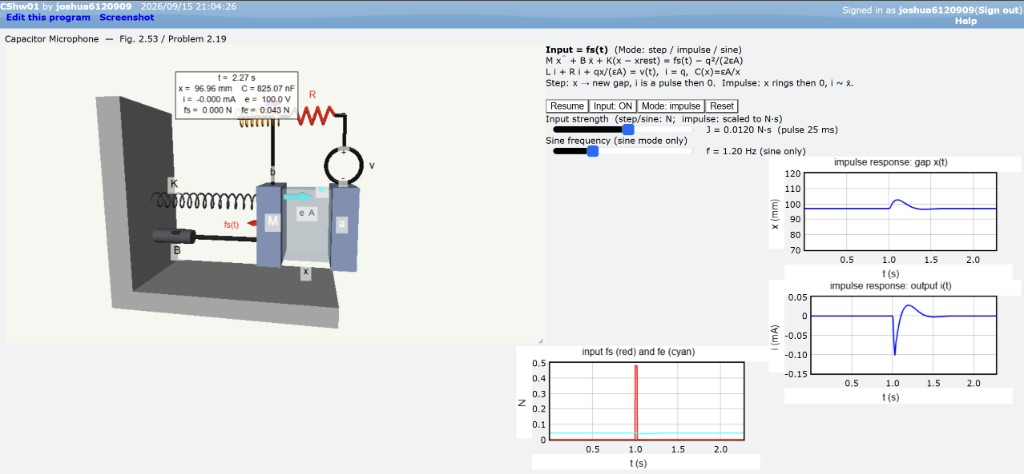
\includegraphics[width=0.88\textwidth,height=0.28\textheight,keepaspectratio]{fig_impulse.png}
  \caption{脈衝響應：\(x\) 晃完回原位，\(i\) 只在運動時非零。}
  \label{fig:impulse}
\end{figure}

\subsection{正弦}

圖~\ref{fig:sine}：聲音改成正弦。\(x\) 和 \(i\) 都持續振盪。
\(f_e\) 幾乎是一條平的線，不會隨速度正負翻轉。

\begin{figure}[ht]
  \centering
  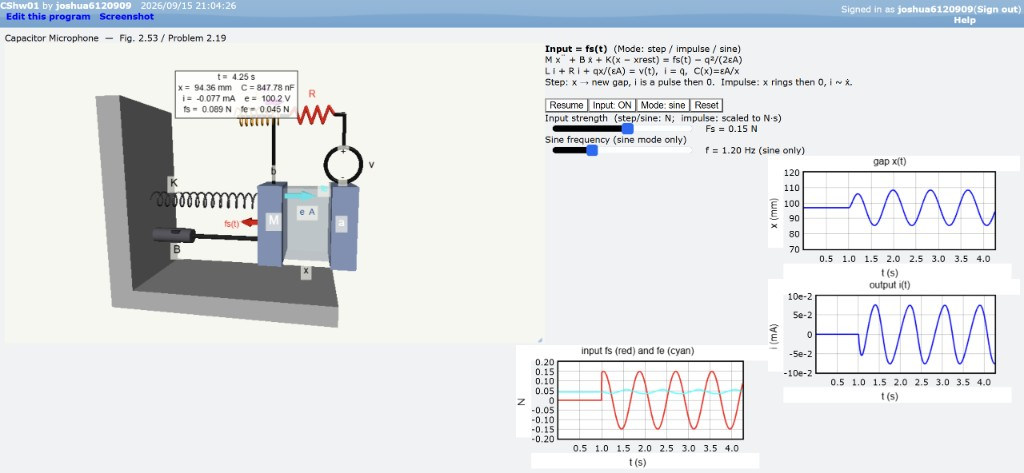
\includegraphics[width=0.88\textwidth,height=0.28\textheight,keepaspectratio]{fig_sine.png}
  \caption{正弦輸入：紅 \(f_s\)、青 \(f_e\)（幾乎恆正）。右圖是 \(x\) 和 \(i\)。}
  \label{fig:sine}
\end{figure}

%==============================================================================
\section{和 \(\operatorname{sgn}\) 模型比一比}

同一組 \(f_s\)、同一組電路，力學差在 \(f_e\) 的方向：
\begin{align}
  \text{物理（藍）}&\quad
  M\ddot{x}+B\dot{x}+K(x-x_{\mathrm{rest}})+f_e=f_s,
  \label{eq:phys}\\
  \text{解答（橘）}&\quad
  M\ddot{x}+B\dot{x}+K(x-x_{\mathrm{rest}})+f_e\operatorname{sgn}(\dot{x})=f_s.
  \label{eq:sol}
\end{align}
兩邊都從「已充電、停在 \(x_{\mathrm{rest}}\)」開始。
\(F_{x,e}\) 是電力沿「張開間隙」的分量，物理上應一直是負的（在吸）。

\subsection{階躍：停著的時候橘色沒有力}

圖~\ref{fig:cstep}，前 \(1.5\,\mathrm{s}\) 沒有聲音：
\begin{itemize}
  \item 藍：一充電就被吸近，\(x\) 從 \(100\,\mathrm{mm}\) 降到約 \(97\,\mathrm{mm}\)。
  \item 橘：\(\operatorname{sgn}(0)=0\)，電力是 0，一直停在 \(100\,\mathrm{mm}\)。
\end{itemize}
板子明明有電，橘色却不動——這不合理。\(1.5\,\mathrm{s}\) 之後才加 step，橘色這才開始動。

\begin{figure}[ht]
  \centering
  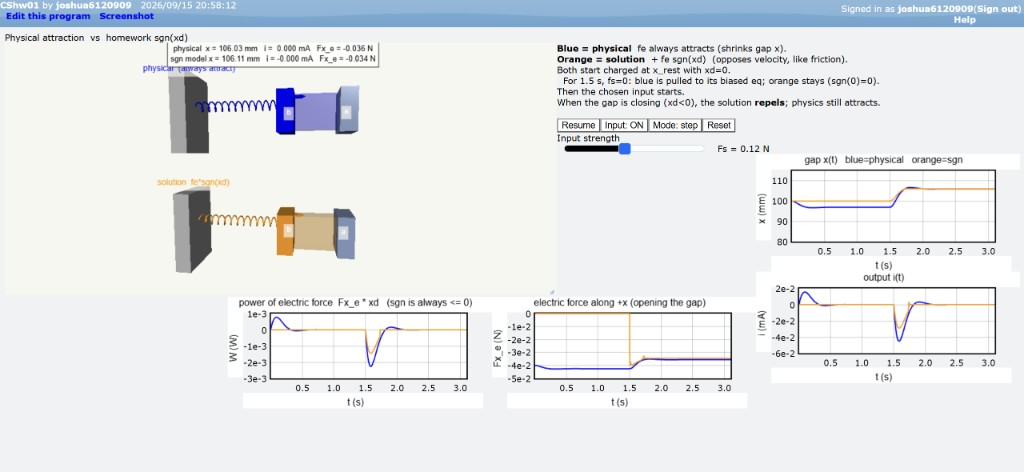
\includegraphics[width=0.88\textwidth,height=0.28\textheight,keepaspectratio]{fig_compare_step.png}
  \caption{藍＝物理，橘＝\(\operatorname{sgn}\)。前 \(1.5\,\mathrm{s}\) 藍色被吸近，橘色不動。}
  \label{fig:cstep}
\end{figure}

\subsection{正弦：力不該跟速度一起翻}

圖~\ref{fig:csine}：
\begin{itemize}
  \item \(x\)：藍色繞較近的平衡點晃；橘色幾乎繞 \(100\,\mathrm{mm}\)（沒有被吸近）。
  \item \(F_{x,e}\)：藍色幾乎是負的直線（一直在吸）；橘色會被速度拉來拉去，常常回到 0。
  \item \(i\)：橘色比較大，因為平均間距和受力都不一樣，輸出也跟著錯。
\end{itemize}

\begin{figure}[ht]
  \centering
  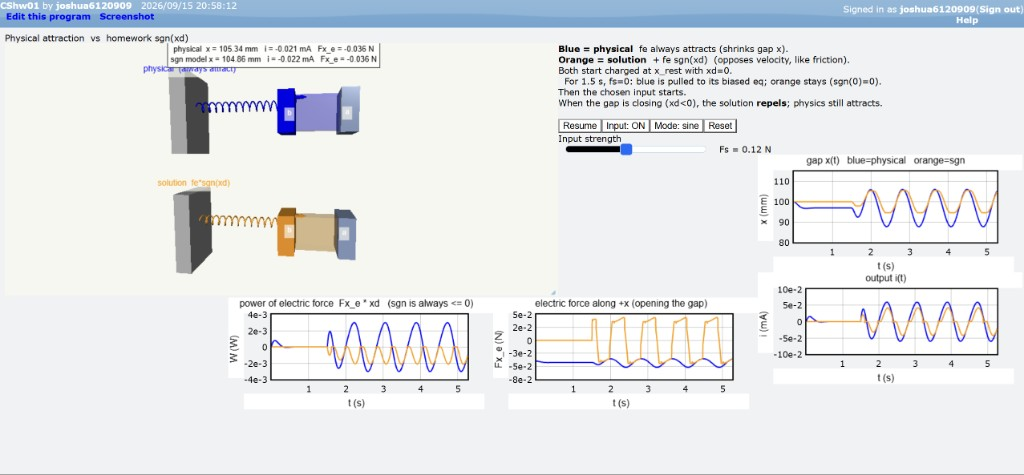
\includegraphics[width=0.88\textwidth,height=0.28\textheight,keepaspectratio]{fig_compare_sine.png}
  \caption{正弦對照。藍色 \(F_{x,e}\) 幾乎恆負；橘色隨速度變，像摩擦不像庫倫力。}
  \label{fig:csine}
\end{figure}

另外，硬的 \(\operatorname{sgn}\) 在速度過零時會讓力正負亂跳（chattering）。
真正的吸引力不該這樣。對照程式裡有做平滑，只是讓圖好看，
「停著無力、靠近变排斥」這兩個錯還在。

%==============================================================================
\section{結論}

\begin{enumerate}
  \item \textbf{(a)} 用 \eqref{eq:nlin}：機械是質量--彈簧--阻尼，外加永遠存在的吸引力；
        電路是間距會變的 \(L\)--\(R\)--\(C\)。
  \item \textbf{(b)} 可以線性化，但要拿掉 \(\operatorname{sgn}\)，並在偏壓點 \((x_0,q_0)\) 做。
        \(q^2\)、\(qx\) 本身可以線性化；解答把它們和 \(\operatorname{sgn}\) 一起說「都不能線性化」過滿。
  \item \textbf{(c)} 輸出是 \(i(t)\)。穩態直流聲音沒有電流；交流時 \(i\) 大約跟 \(\dot{x}\) 成正比。
  \item \(\operatorname{sgn}(\dot{x})\) 和題目的 \(f_e=q^2/(2\varepsilon A)\) 對不上：
        兩板異號，力應一直吸引。模擬也顯示：靜止時橘色沒有力，正弦時力會跟速度翻轉。
\end{enumerate}

“opposes its motion” 應讀成「拉開要克服吸力」。
方程式請用 \eqref{eq:mech}，不要用 \eqref{eq:sgn}。

\vspace{0.8em}
\noindent 程式：\texttt{capacitor\_microphone.py}（物理）、
\texttt{capacitor\_microphone\_sgn\_compare.py}（對照）。

\end{document}
